\chapter{Autoregulon Networks: COMING SOON}
\label{ch-autoregulons}

Appendix \ref{ch-genomics-vocab}

\section{Autoregulon net motif}
a {\bf net motif} is just a subgraph of a bnet

\begin{figure}[h!]
$$
\xymatrix{
&\rvx\ar[dd]|{-\alp}\ar[dl]
\\
f(\rvx)\ar[dr]|{1}
\\
&\Circle{\frac{d\rvx}{dt}}
}\quad
\xymatrix{\\=}
\quad
\xymatrix{
\\
\rvx\ar@{=>}[d]
\\
\dot{\rvx}
}
$$
\caption{Autoregulon net motif and the symbol we will
use to denote it when we consider
networks of connected autoregulons. Assume $\alp >0$.}
\label{fig-net-motif}
\end{figure}

\beq
\frac{dx}{dt}=f(x)-\alp x
\eeq

\beq
f(x)=\left\{
\begin{array}{ll}
\beta\indi(x<K)
&(f \text{ is lowpass})
\\
\beta\indi(x>K)
&(f \text{ is highpass})
\end{array}
\right.
\eeq
where $\alp, \beta > 0$

\hrule
For $f$ lowpass
\beq
x= 
\left\{
\begin{array}{ll}
x_0 e^{-\alp t} +
\frac{\beta}{\alp}\left[1-e^{-\alp t}\right]
&\text{ if } t<t_K
\\
x_K e^{-\alp (t-t_K)}
&\text{ if } t>t_K
\end{array}
\right.
\eeq
where, to make $x(t)$ continuous at $t=t_K$ and $x(t_K)=x_K$,
we must have

\beq
 x_0 e^{-\alp t_K} +
\frac{\beta}{\alp}
\left[1-e^{-\alp t_K}\right]
=
x_K
\eeq

Note that if $\alp t<<1$, then\footnote{Use $e^x\approx 1 + x$ for $|x|<<1$.}, 

\beqa
x &\approx&
x_0(1-\alp t) +\beta t
\\ &=&
x_0 + (\beta -\alp x_0)t
\eeqa

Assume $x_0=0$ for simplicity.
In that case, if $K>\frac{\beta} {\alp}$, $t_K$ 
doesn't exist and only the $t<t_K$
branch of the $x$ solution above exists.
On the other hand, if $K<\frac{\beta} {\alp}$, 
then $t_K$ exists and $x_K=K$.
For $t>t_K$,

\beq
x=
K e^{-\alp(t-t_K)}
\eeq

\begin{figure}[h!]
\centering
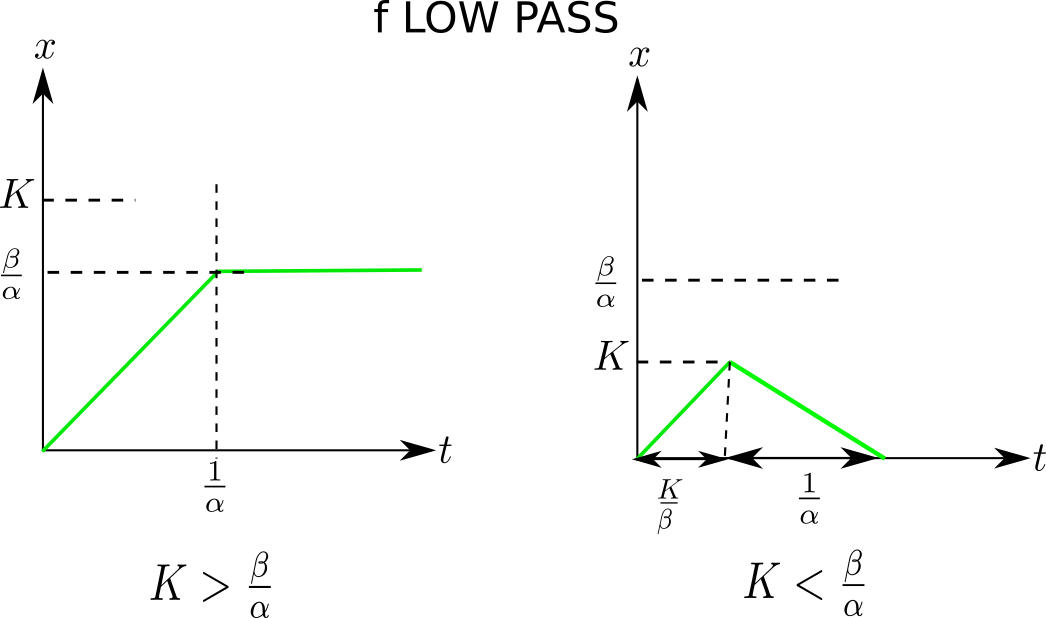
\includegraphics[width=4in]
{autoregulons/autoreg-lowpass.png}
\caption{Approximate $x$ for autoregulon with lowpass $f$
and $x_0=0$}
\label{fig-autoreg-lowpass}
\end{figure}

See Fig.\ref{fig-autoreg-lowpass}
for approximate 
$x$ for autoregulon with lowpass $f$
and $x_0=0$.


\hrule
For $f$ highpass

\beq
x= 
\left\{
\begin{array}{ll}
x_0 e^{-\alp t} &\text{ if } t<t_K  
\\
x_K e^{-\alp (t-t_K)} +
\frac{\beta}{\alp}
\left[ 1-e^{-\alp (t-t_K)}\right]
&\text{ if } t>t_K
\end{array}
\right.
\eeq
where, to make $x(t)$ continuous at $t=t_K$ and $x(t_K)=x_K$,
we must have

\beq
x_0 e^{-\alp t_K} = x_K
\eeq

Note that if $\alp t<<1$, then

\beqa
x &\approx&
x_0(1 -\alp t)
\eeqa
Unlike when $f$ is lowpass, 
in this case of $f$ highpass,
we can't assume $x_0=0$ or else $x_K=K=0$ too. In fact, we must have $x_0 > x_K=K$. For $\alp (t-t_K) >>1$, 
\beq
x\approx \frac{\beta}{\alp}
\eeq

\begin{figure}[h!]
\centering
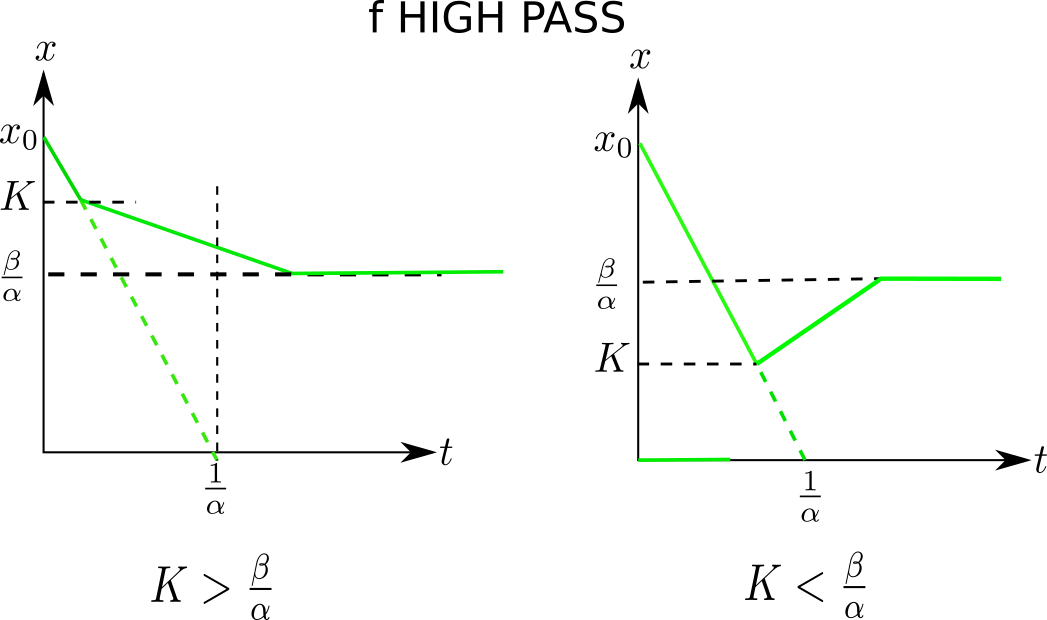
\includegraphics[width=4in]
{autoregulons/autoreg-highpass.png}
\caption{Approximate $x$ for autoregulon with highpass $f$}
\label{fig-autoreg-highpass}
\end{figure}
See Fig.\ref{fig-autoreg-highpass}
for picture of 
approximate $x$ for autoregulon with highpass $f$.

\hrule


Three $x$ values $\{x_0, K, \frac{\beta}{\alp}\}$, and
two $f$ values $\{ \text{lowpass, highpass}\}$






\section{Multiple autoregulons}

\beq
\cala x = 0\;,\;\; \text{ where } \cala=
\frac{d}{dt} + \alp - \frac{f(x)}{x}
\eeq





\begin{figure}[h!]
$$
\xymatrix@C=6pc{
\rvx \ar@{=>}[dd]\ar[ddr]^<<<<{\gamma_{\rvy|\rvx}}
& \rvy \ar@{=>}[dd]\ar[ddl]_<<<<{\gamma_{\rvx|\rvy}}
\\
&
\\
\dot{\rvx}
&\dot{\rvy}
}
\xymatrix{\\
\quad=\quad}
\xymatrix@C=5pc{
\\
\Rect{\rvx}
\autoar{r}
{\gamma_{\rvy|\rvx}}
{\gamma_{\rvx|\rvy}}
&
\Rect{\rvy}}
$$
\caption{Two autoregulons connected to each other.}
\label{fig-2-autoregulons}
\end{figure}

\beq
\left\{
\begin{array}{l}
\cala\rvx = \gamma_{\rvx|\rvy}\;\rvy
\\
\cala\rvy = \gamma_{\rvy|\rvx}\;\rvx
\end{array}
\right.
\eeq


\begin{figure}[h!]
$$
\xymatrix@C=4pc@R=5pc{
&\Rect{\rvx}
\autoar{ld}{}{}
\autoar{rd}{}{}
\\
\Rect{\rvy}\autoar{rr}{}{}
&&
\Rect{\rvz}
}
$$
\caption{Three autoregulons connected to each other.
$\gamma_{\rvx|\rvy}$ coefficients are left implicit.}
\label{fig-3-autoregulons}
\end{figure}


\beq
\left\{
\begin{array}{l}
\cala\rvx =
\gamma_{\rvx|\rvy}\;\rvy
+
\gamma_{\rvx|\rvz}\;\rvz
\\
\cala\rvy =
\gamma_{\rvy|\rvx}\;\rvx
+
\gamma_{\rvy|\rvz}\;\rvz
\\
\cala\rvz =
\gamma_{\rvz|\rvx}\;\rvx
+
\gamma_{\rvz|\rvy}\;\rvy
\end{array}
\right.
\eeq

Use $\xymatrix{\rvx\ar[r]^{+}&\rvy}$
to denote
$\xymatrix{\rvx\ar[r]^\alp&\rvy}$
with $\alp>0$.

Use $\xymatrix{\rvx\ar[r]^{-}&\rvy}$
to denote
$\xymatrix{\rvx\ar[r]^\alp&\rvy}$
with $\alp<0$

Use $\xymatrix{\rvx\ar[r]^{0}&\rvy}$
to denote
$\xymatrix{\rvx\ar[r]^\alp&\rvy}$
with $\alp=0$.

\begin{figure}[h!]
$$
\begin{array}{ccc}
\xymatrix@C=4pc@R=5pc{
&\Rect{\rvx}
\autoar{ld}{-}{0}
\autoar{rd}{+}{0}
\\
\Rect{\rvy}\autoar{rr}{-}{0}
&&
\Rect{\rvz}
}
&&
\xymatrix@C=4pc@R=5pc{
&\Rect{\rvx}
\autoar{ld}{-}{0}
\autoar{rd}{+}{0}
\\
\Rect{\rvy}\autoar{rr}{+}{0}
&&
\Rect{\rvz}
}
\\
\\
(a)&&(b)
\end{array}
$$
\caption{$(a)$ shows a coherent net of 3 autoregulons because $\sign(\gamma_{\rvz|\rvy}\gamma_{\rvy|\rvx})=\sign(\gamma_{\rvz|\rvx})$.
$(b)$ shows a incoherent net of 3 autoregulons because $\sign(\gamma_{\rvz|\rvy}\gamma_{\rvy|\rvx})\neq \sign(\gamma_{\rvz|\rvx})$.
}
\label{fig-3-coherent-autoregulons}
\end{figure}



\section{Single Input Module (SIM) net}

\section{Feedforward Loop (FFL) net}

\section{Bistable net}

\section{Biological clock net}